%<dscrpt>Droites, cercles : géométrie élémentaire avec des complexes. </dscrpt>
Dans tout le problème \footnote{d'après concours général 2005}, on se place dans un plan $\mathcal P$ muni d'un repère orthonormé direct $(O,\overrightarrow{i},\overrightarrow{j})$ et on convient de désigner les points avec des capitales et les affixes avec des minuscules. Par exemple, l'affixe d'un point $M$ sera le complexe $m$, le représentant d'un nombre complexe $z$ sera le point $Z$.\newline
Soit $A$ et $B$ deux points distincts.\newline
Rappelons la définition d'une symétrie par rapport à une droite. Les points $M$ et $M'$ sont dits symétriques par rapport à la droite $(AB)$ si et seulement si:
\begin{center}
  le milieu de $M$ et $M'$ appartient à $(AB)$ et $\overrightarrow{M M'}$ est orthogonal à $\overrightarrow{AB}$.
\end{center}
\begin{figure}[!ht]
  \centering
  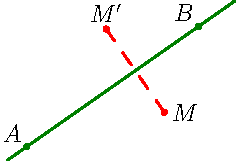
\includegraphics{Ecomp2_0.pdf}
  % Ecomp2_0.pdf: 142x104 px, 72dpi, 5.01x3.67 cm, bb=0 0 142 104
  \caption{Points symetriques par rapport à $(AB)$}
  \label{fig:Ecomp2_0}
\end{figure}
Rappelons aussi la définition de la médiatrice d'un segment. L'ensemble des points à égale distance de $A$ et de $B$ est une droite appelée médiatrice de $AB$.

\subsection*{Partie I. Expression complexe d'une symétrie} \noindent
Soit $A$ et $B$ deux points distincts d'affixes complexes $a$ et $b$ avec $a\neq b$.
\begin{enumerate}
  \item 
  \begin{enumerate}
    \item Donner la définition du nombre complexe $j$ et ses premières propriétés, calculer 
\[
  \frac{j^2 - j}{\overline{j^2 - j}}.
\]

    \item Soit $u$ un nombre complexe non nul. Montrer que les points d'affixes $u$, $ju$, $j^2u$ forment un triangle équilatéral.
  \end{enumerate}

  \item Soit $M$ et $M'$ (d'affixes $m$ et $m'$) deux points symétriques par rapport à $(AB)$.
  \begin{enumerate}
    \item Montrer qu'il existe $\lambda \in \R$ tel que 
    \[
      m' + m = 2a + 2(b-a)\lambda.
    \]
    \item Montrer qu'il existe $\mu \in \R$ tel que 
    \[
      m' - m = \mu i (b-a).
    \]
    \item En déduire
    \[
      \frac{m' - a}{b - a} = \overline{\left(\frac{m - a}{b-a}\right)}.
    \]
  \end{enumerate}

  \item Soit $w_1$ et $w_2$ complexes. On définit la fonction $s$ de $\C$ dans $\C$ par:
  \[
    \forall z \in \C, \; s(z) = w_1 \overline{z} + w_2.
  \]
  \begin{enumerate}
    \item En utilisant les formules de Cramer, calculer $w_1$ et $w_2$ tels que $s(a)=a$ et $s(b)=b$.
    \item Pour $z\in \C$, on note $z' = s(z)$ et $Z$, $Z'$ les points d'affixe $z$ et $z'$. Vérifier que $Z$ et $Z'$ sont symétriques par rapport à $(AB)$.
  \end{enumerate}
\end{enumerate}

\begin{figure}[!ht]
 \centering
 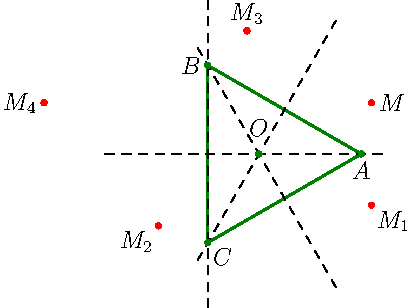
\includegraphics[width=5.5cm]{Ecomp2_1.pdf}
 \caption{Points $M$, $M_1$, $M_2$, $M_3$, $M_4$}
 \label{fig:Ecomp2_1}
\end{figure}

\subsection*{Partie II} \noindent
On considère les points $O$, $A$, $B$, $C$ respectivement d'affixes $0$, $1$, $j$, $j^2$.\newline
Soit $M$ un point d'affixe $m \neq 0$. On note $\rho = \vert m \vert$ et $\theta$ un argument de $m$.\newline
Soit $M_1$, $M_2$, $M_3$, $M_4$ les points symétriques de $M$ respectivement par rapport aux droites $(OA)$, $(OB)$, $(OC)$ et $(BC)$.
\begin{figure}[ht]
 \centering
 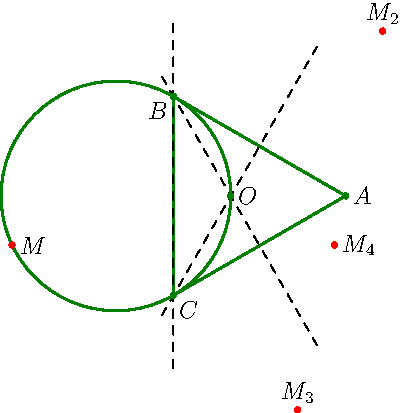
\includegraphics[width=5.5cm]{Ecomp2_2.pdf}
 \caption{Alignement de $M_2$, $M_3$, $M_4$}
 \label{fig:Ecomp2_2}
\end{figure}

\begin{enumerate}
 \item Calculer $m_1$, $m_2$, $m_3$, $m_4$ en fonction de $m$. Montrer que $M_1$, $M_2$, $M_3$ est équilatéral.
 \item Montrer que $M_2$, $M_3$, $M_4$ sont alignés si et seulement si $M$ est sur un certain cercle à préciser. Vérifier que, dans ce cas, le point $A$ est aussi sur la droite qui contient $M_2$, $M_3$, $M_4$.
 \item Si $M_2$, $M_3$, $M_4$ ne sont pas alignés, il existe un cercle (appelé cercle circonscrit) qui contient ces trois points.  On note $\Omega$ (d'affixe $\omega$) le centre de ce cercle et $R$ son rayon. On pourra utiliser que le point $\Omega$ est l'intersection des médiatrices des segments $M_2 M_3$, $M_2 M_4$, $M_3 M_4$.
    \begin{enumerate}
     \item Montrer que $O$ et $M_1$ appartiennent à la médiatrice de $M_2 M_3$. En déduire qu'il existe $\lambda$ réel tel que $\omega = \lambda e^{-i \theta}$.
     \item En utilisant le fait que $\Omega$ appartient à la médiatrice de $M_2 M_3$, montrer que
 \[
 \omega = - \frac{1+2\rho \cos \theta}{\rho +2 \cos \theta} \, e^{-i \theta}.
 \]
     \item Montrer que 
\[
  R^2= \rho^2 +\frac{(1-\rho^2)(1+2\rho \cos \theta)}{(\rho + 2 \cos \theta)^2}.
\]
    \end{enumerate}

\item Préciser géométriquement l'ensemble $\Gamma$ des points $M$ tels que les cercles circonscrits à $M_1$, $M_2$, $M_3$ et à $M_2$, $M_3$, $M_4$ aient les mêmes rayons.\newline
Reproduire approximativement, compléter et interpréter les figures~\ref{fig:Ecomp2_3} et \ref{fig:Ecomp2_4} des configurations 1 et 2.
\end{enumerate}

\begin{figure}[ht]
 \centering
 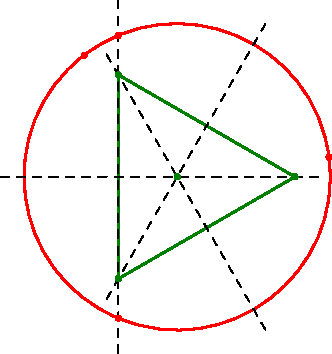
\includegraphics[width=4cm]{Ecomp2_3.pdf}
 \caption{Configuration 1}  \label{fig:Ecomp2_3}
\end{figure}
\begin{figure}[ht]
 \centering
 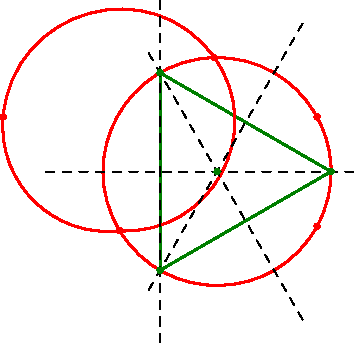
\includegraphics[width=4cm]{Ecomp2_4.pdf}
  \caption{Configuration 2}\label{fig:Ecomp2_4}
\end{figure}

\clearpage

